\documentclass[a4paper,12pt]{article}

\usepackage{mystyle}
\usepackage{gensymb}


\usepackage{scalerel}
\usepackage{stackengine}

\graphicspath{ {images/} }


% https://tex.stackexchange.com/questions/5461/is-it-possible-to-change-the-size-of-an-arrowhead-in-tikz-pgf
\usetikzlibrary{arrows.meta}


\DeclareMathOperator{\Image}{Im}
\definecolor{violet}{RGB}{148, 0, 211}
\definecolor{green}{RGB}{0, 153, 0}
\definecolor{orange}{RGB}{255, 153, 0}
\definecolor{blue}{RGB}{31, 117, 254}


% https://tex.stackexchange.com/a/101138/135045

\newcommand\widesim[1]{\ThisStyle{%
  \setbox0=\hbox{$\SavedStyle#1$}%
  \stackengine{-.1\LMpt}{$\SavedStyle#1$}{%
    \stretchto{\scaleto{\SavedStyle\mkern.2mu\sim}{.5150\wd0}}{.6\ht0}%
  }{O}{c}{F}{T}{S}%
}}

\newcommand{\BigMiddleThree}{\;\left|\vphantom{\begin{pmatrix} 0\\0\\0 \end{pmatrix}}\right.\;}
\newcommand{\BigMiddleFour}{\;\left|\vphantom{\begin{pmatrix} 0\\0\\0\\0 \end{pmatrix}}\right.\;}


% https://tex.stackexchange.com/questions/63531/how-to-write-quotation-marks-in-math-environment
\DeclareMathSymbol{\mlq}{\mathord}{operators}{``}
\DeclareMathSymbol{\mrq}{\mathord}{operators}{`'}


\DeclareMathOperator{\Imag}{Im}


% https://tex.stackexchange.com/questions/544453/undefined-control-sequence-after-paragraph
\renewcommand{\paragraph}[1]{\noindent\textbf{#1}\quad}

% https://tex.stackexchange.com/questions/36851/skipping-line-after-proof-in-proof-environment#comment73553_36851
\newcommand{\proofindent}{\hspace*{\fill}\par\vspace{0.5em}}


\author{Алексеев Василий}


\title{Семинар 5}
\date{7 + 10 марта 2023}


\begin{document}
  \maketitle
  
  \tableofcontents

  \thispagestyle{empty}
  
  \newpage
  
  \pagenumbering{arabic}


  \section{Линейные отображения 1}
  
  \subsection{Отображение. Инъективность и сюръективность}
  
  Об \emph{отображении} $\phi\colon X \hm\to Y$ можно думать как о правиле, которое \emph{каждому} элементу множества $X$ ставит в соответствие \emph{единственный} элемент множества $Y$\footnote{Множество $X$ в таком случае называется \emph{областью определения} отображения $\phi$ (множество ``допустимых'' входов). Таким образом, область определения~---~это часть определения отображения (определение области определения отображения~---~``тот самый $X$'' из определения отображения). Поэтому, когда в ``школьных'' номерах по математике просили ``найти область определения функции'', то имели в виду найти ``максимально возможное по количеству элементов множество, которое могло бы выступать в роли области определения функции'' (если бы привели полноценное определение этой функции, а не просто формулу).}~(\ref{fig:function}).
  Если отображение $\phi$ переводит элемент $x \hm\in X$ в элемент $y \hm\in Y$, то можно записать $\phi(x) \hm= y$, при этом $y$ называется \emph{образом} $x$, а $x$~---~прообразом $y$ (одним из возможных, если их несколько).
  
  \begin{figure}[h]
    \centering
  
    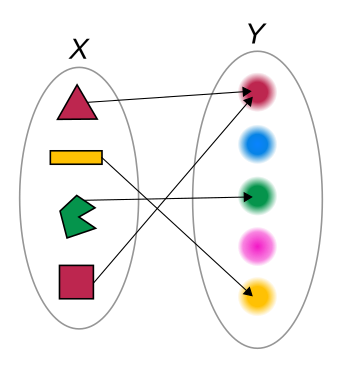
\includegraphics[width=0.3\columnwidth]{function}
  
    \caption{Отображение: каждому элементу $X$ соответствует единственный элемент $Y$ (источник картинки: \href{https://en.wikipedia.org/wiki/Function\_(mathematics)\#/media/File:Function_color_example_3.svg}{Википедия}).}
    \label{fig:function}
  \end{figure}
  
  % Про область определения:
  % https://math.stackexchange.com/a/2912118/451127
  % https://math.stackexchange.com/questions/63043/finding-a-functions-domain-from-the-functions-formula/63048#63048
  
  Можно отметить несколько свойств, которыми могут обладать произвольные отображения.
  
  \begin{definition}
    Отображение~$\phi$ называется \emph{инъективным}, если разные элементы отображаются в разные~(\ref{fig:injection}):
    $
      x_1, x_2 \hm\in X,\ x_1 \hm{\not=} x_2 \hm\Rightarrow \phi(x_1) \hm{\not=} \phi(x_2)
    $.
    Иными словами, если у элемента $y \hm\in Y$ есть прообраз, то он единственный.
  \end{definition}
  
  \begin{definition}
    Отображение~$\phi$ называется \emph{сюръективным}, если у \emph{любого} элемента $y \hm\in Y$ есть прообраз~(\ref{fig:surjection}):
    $
      \forall y \in Y\ \exists x \in X\colon \phi(x) = y
    $.
  \end{definition}
  
  \begin{figure}[h]
    \centering
    
    \begin{subfigure}[b]{0.3\textwidth}
      \centering
    
      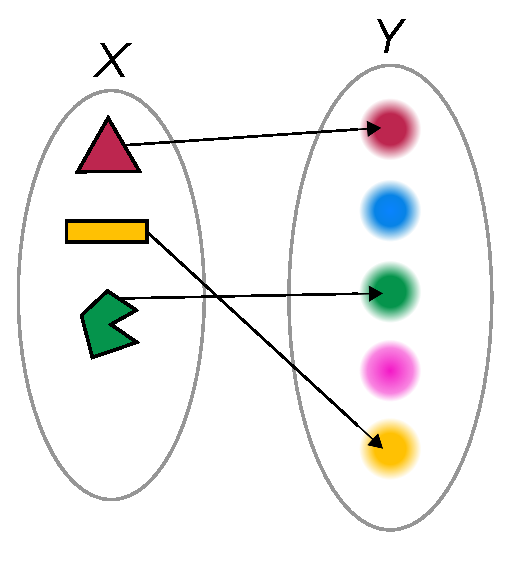
\includegraphics[width=\columnwidth]{injection}
    
      \caption{Инъекция.}
      \label{fig:injection}
    \end{subfigure}
    \hspace{2em}
    \begin{subfigure}[b]{0.3\textwidth}
      
      \centering
      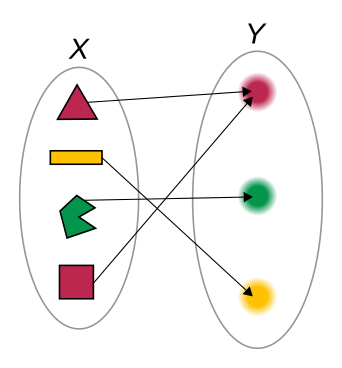
\includegraphics[width=\columnwidth]{surjection}
  
      \caption{Сюръекция.}
      \label{fig:surjection}
    \end{subfigure}
    
    \caption{Инъекция: ``разные в разные'', или ``если есть прообраз, то один''. Сюръекция: ``у~каждого есть хотя бы один прообраз''.}
  \end{figure}
  
  Факт наличия у отображения обоих приведённых выше свойств сразу выделяется в отдельное свойство.
  
  \begin{definition}
    Отображение~$\phi$ называется \emph{биективным}, если у \emph{любого} элемента $y \hm\in Y$ есть \emph{единственный} прообраз:
    $
      \forall y \in Y\ \exists ! x \in X\colon \phi(x) = y
    $.
  \end{definition}
  
  Помимо множества $X$ (области определения отображения $\phi$, или domain), и множества $Y$ (для которого, похоже, в русском языке нет специального названия, а по-английски~---~codomain) можно выделить ещё одно ``интересное'' множество, связанное с отображением~$\phi$~--- это \emph{множество значений} отображения $\Imag \phi \hm\subseteq Y$, которое определяется как совокупность всех элементов $y \hm\in Y$, в которые в принципе ``можно попасть'' под действием отображения:
  \[
    \Imag \phi = \{y \in Y \mid \exists x \in X\colon \phi(x) = y\}
  \]
  
  Тогда сюръективность означает, что $\Imag \phi \hm= Y$.
  
  
  \subsection{Линейное отображение. Ядро и множество значений}
  
  % Footnotes: https://tex.stackexchange.com/a/35060/135045
  
  \begin{definition}
    Пусть $X$ и $Y$~---~линейные пространства, размерностей $n$ и $m$ соотвественно (возможно, разных).
    Тогда отображение\footnote{Начиная с этого определения и далее в конспекте векторы ``абстрактных'' пространств $X$ и $Y$ будут обозначаться жирным шрифтом, чтобы их проще было отличать от ``обычных'' числовых вектор-столбцов, которые далее ещё появятся.} $\phi\colon X \to Y$ называется \emph{линейным}, если
    \begin{itemize}
      \item $\phi(\bds x_1 + \bds x_2) \hm= \phi(\bds x_1) \hm+ \phi(\bds x_2), \quad \forall \bds x_1, \bds x_2 \hm\in X$
      \item $\phi(\alpha \bds x) \hm= \alpha \phi(\bds x),\quad \forall \alpha \hm\in \RR,\ \bds x \hm\in X$
    \end{itemize}
  \end{definition}
  
  Далее отметим несколько небезынтересных утверждений, связанных именно с линейными отображениями.
  Но сначала введём ещё одно понятие (которое можно ввести в виду того, что $X$ и $Y$ линейные пространства).
  
  \begin{definition}
    \emph{Ядром} отображения\footnote{В этом разделе отображение иногда может упоминаться просто как ``отображение $\phi$''~---~имеется в виду именно $\phi\colon X \hm\to Y$, то есть отображение из линейного пространства $X$ в линейное пространство $Y$.} $\phi$ называется подмножество элементов $\Ker\phi \hm\subseteq X$, которые в результате действия $\phi$ отображаются в нулевой элемент пространства~$Y$:
    \[
      \Ker \phi = \{\bds x \in X \mid \phi(\bds x) = \bds 0\}
    \]
  \end{definition}
  
  \begin{proposition}
    $\Ker \phi$ есть линейное подпространство в $X$.
  \end{proposition}
  
  \begin{proof}
    Покажем это, проверив замкнутость относительно операций сложения и умножения на число (которые определены в линейном пространстве~$X$).
    Пусть $\bds x_1, \bds x_2 \hm\in \Ker \phi$, то есть $\phi(\bds x_1) \hm= \bds 0$ и $\phi(\bds x_2) \hm= \bds 0$.
    Тогда, пользуясь линейностью $\phi$, можем расписать, чему равен образ суммы $\bds x_1 \hm+ \bds x_2$:
    \[
      \phi(\bds x_1 + \bds x_2) = \phi(\bds x_1) + \phi(\bds x_2) = \bds 0 + \bds 0 = \bds 0 \Rightarrow \bds x_1 + \bds x_2 \in \Ker \phi
    \]
    
    Аналогично, образ вектора, полученного умножением произвольного вектора $\bds x$ из ядра на число $\alpha \hm\in \RR$:
    \[
      \phi(\alpha \bds x) = \alpha \phi(\bds x) = \alpha \bds 0 = \bds 0 \Rightarrow \alpha \bds x \in \Ker \phi
    \]
  \end{proof}
  
  Раз ядро подпространство, то в нём как минимум есть нулевой вектор пространства~$X$.
  (И это не сложно показать.)
  С ядром также связан возможный способ проверки инъективности отображения.
  
  \begin{proposition}[``Критерий инъективности'']
    \proofindent
    Отображение $\phi$ инъективно $\Leftrightarrow$ его ядро нулевое: $\Ker \phi \hm= \{\bds 0\}$.
  \end{proposition}
  
  \begin{proof}
    ``Слева-направо''.
    Пусть отображение инъективно.
    Покажем, что тогда обязательно ядро нулевое.
    Допустим, что это не так, то есть $\exists \bds x^* \hm\in \Ker \phi$, $\bds x^* \hm{\not=} \bds 0$.
    Как отсюда получить противоречие с инъективностью?
    Инъективно~---~``разные в разные''.
    Пусть $\bds x \hm\in X$.
    Тогда
    \[
      \phi(\bds x + \bds x^*) = \phi(\bds x) + \phi(\bds x^*) = \phi(\bds x)
    \]
    то есть образы $\bds x \hm+ \bds x^*$ и $\bds x$ совпадают, но сами векторы разные, так как $\bds x^*$ ненулевой.
    А при инъективном отображении такого не может быть.
    
    ``Справа-налево''.
    Пусть ядро отображения нулевое.
    Покажем, что при этом отображение обязательно инъективно.
    Снова предположим, что это не так, то есть найдутся $\bds x_1$ и $\bds x_2$, $\bds x_1 \hm{\not=} \bds x_2$, но $\phi(\bds x_1) \hm= \phi(\bds x_2)$.
    Раз так, то, пользуясь линейностью $\phi$, получаем:
    \[
      \bds 0 = \phi(\bds x_1) - \phi(\bds x_2) = \phi(\bds x_1 - \bds x_2) \Rightarrow \bds x_1 - \bds x_2 \in \Ker \phi
    \]
    но $\bds x_1 \hm- \bds x_2 \hm{\not=} \bds 0$, то есть нашли ненулевой элемент в ядре.
    А по условию такого не может быть.
  \end{proof}
  
  \begin{proposition}
    $\Imag \phi$ есть линейное подпространство в $Y$.
  \end{proposition}
  
  \begin{proof}
    Аналогично проверке того, что ядро подпространство~---~здесь тоже можно показать замкнутость множества значений, но уже в линейном пространстве~$Y$ (относительно операций сложения и умножения на число, определённых в~$Y$).
    Пусть есть векторы $\bds y_1, \bds y_2 \hm\in Y$.
    Это значит, что у каждого из них есть прообраз (хотя бы один), то есть найдутся $\bds x_1, \bds x_2 \hm\in X$, такие что $\phi(\bds x_1) \hm= \bds y_1$ и $\phi(\bds x_2) \hm= \bds y_2$.
    Посмотрим на сумму $\bds y_1 \hm+ \bds y_2$~---~будет ли она в $\Imag \phi$?
    Да, имея в виду линейность $\phi$, несложно найти её возможный прообраз:
    \[
      \phi(\bds x_1 + \bds x_2) = \phi(\bds x_1) + \phi(\bds x_2) = \bds y_1 + \bds y_2 \Rightarrow \bds y_1 + \bds y_2 \in \Imag \phi
    \]
    
    Точно так же с умножением на число $\alpha \hm\in \RR$ произвольного вектора $\bds y \hm\in \Imag \phi$, в который отображается, например, вектор $\bds x \hm\in X$:
    \[
      \phi(\alpha \bds x) = \alpha \phi(\bds x) = \alpha \bds y \Rightarrow \alpha \bds y \in \Imag \phi
    \]
  \end{proof}
  
  Раз множество значений отображения является подпространством~$Y$, то несложно прийти к такому способу проверки сюръективности.
  
  \begin{proposition}[``Критерий сюръективности'']
    \proofindent
    Отображение $\phi$ сюръективно $\Leftrightarrow \dim\Imag\phi \hm= \dim Y$.
  \end{proposition}
  
  Если размерность подпространства совпадает с размерностью всего пространства, то, очевидно, подпространство и есть пространство (например, трёхмерное ``подпространство'' в геометрическом пространстве векторов трёхмерного пространства).
  Но $\Imag \phi \hm= Y$ и есть суть сюръективности.
  
  Сравнение размерностей в самом деле удобный способ, потому что как бы ещё можно было проверить сюръективность?
  Перебирать все $\bds y \in Y$ и искать прообраз?
  А так~---~можно выбрать базис в $Y$, найти базис в $\Imag \phi$, сравнить числа векторов в базисах, и из этого сразу будет понятно, сюръективно $\phi$ или нет.
  
  
  \subsection{Матрица линейного отображения}
  \label{sec:plot1}
  
  Выберем базисы~(\ref{fig:map-maps-map-to-map}) в пространствах $X$ и $Y$: строчки из базисных векторов $e \hm= (\bds e_1, \ldots, \bds e_n) \hm\subset X$ и $f \hm= (\bds f_1, \ldots, \bds f_m) \hm\subset Y$ (считаем $n \hm> 0$ и $m \hm> 0$).
  Рассмотрим действие отображения $\phi$ на вектор $\bds x \hm\in X$, столбец компонент которого в базисе $e$ есть $\xi \hm= (x_1, \ldots, x_n)^T$:
  \begin{equation*}
  \begin{split}
    \phi(\bds x) = \phi(x_1 \bds e_1 + \ldots + x_n \bds e_n)
    = x_1 \phi(\bds e_1) + \ldots + x_n \phi(\bds e_n)
    = \underbrace{\bigl(\phi(\bds e_1), \ldots, \phi(\bds e_n)\bigr)}_{\substack{\mbox{\small строка}\\ \mbox{\small векторов}}} \underbrace{\begin{pmatrix}
      x_1 \\ \vdots \\ x_n
    \end{pmatrix}}_{\substack{\mbox{\small столбец}\\ \mbox{\small координат}}}
  \end{split}
  \end{equation*}
  
  Вектор, например, $\phi(\bds e_1) \hm\in Y$ также можно разложить по базису, но уже по базису $f$:
  \[
    \phi(\bds e_1) = a_{11} \bds f_1 + \ldots + a_{m1} \bds f_m = (\bds f_1, \ldots, \bds f_m) \begin{pmatrix}
      a_{11} \\ \vdots \\ a_{m1}
    \end{pmatrix}
  \]
  
  Обозначим символом $a_1 \hm\in \RR^m$ вектор-столбец $(a_{11}, \ldots, a_{m1})^T$ координат вектора $\phi(\bds e_1)$ в базисе $f$\footnote{В обозначениях рисунка~(\ref{fig:map-maps-map-to-map}) $\phi(e_1)$ это $\widetilde\phi\bigl( h_X(\bds e_1) \bigr)$.}.
  
  Таким образом, возвращаясь к вычислению образа вектора~$\bds x$:
  \begin{equation*}
    \phi(\bds x)
    = \bigl(\phi(\bds e_1), \ldots, \phi(\bds e_n)\bigr) \begin{pmatrix}
      x_1 \\ \vdots \\ x_n
    \end{pmatrix}
    = (\bds f_1, \ldots, \bds f_m) \underbrace{\bigl(a_1, \ldots, a_n\bigr)}_{A \in \RR^{m \times n}} \begin{pmatrix}
      x_1 \\ \vdots \\ x_n
    \end{pmatrix}
    = f A \xi
  \end{equation*}
  
  С другой стороны, так как вектор $\phi(\bds x) \hm\in Y$, то он раскладывается по базису $f$ с некоторыми коэффициентами $\eta \hm= (y_1, \ldots, y_m)^T$:
  \[
    \phi(\bds x) = (\bds f_1, \ldots, \bds f_m) \begin{pmatrix}
      y_1 \\ \vdots \\ y_m
    \end{pmatrix}
    = f \eta
  \]
  
  Получили два представления одного и того же вектора $\phi(\bds x)$:
  \begin{equation}\label{eq:double-faced-phi-x}
    f \eta = f A \xi \xrightarrow{f\, \mbox{\scriptsize базис}} \boxed{\eta = A \xi}
  \end{equation}
  
  Матрица $A$ называется \emph{матрицей линейного отображения} в паре базисов $e$ и $f$.
  
  \begin{figure}[h]
    \centering
    
    % https://tex.stackexchange.com/a/75450/135045
    \resizebox{0.35\textwidth}{!}{%
      \begin{tikzpicture}
        \node[anchor=south] at (0,0) {$\bds x$};
        \coordinate (A) at (0,0);
        
        \node[anchor=south] at (-0.6,0) {$X \ni$};  % TODO: align text in node
        
        \node[anchor=south] at (0.8,0) {$\overset{\phi}{\mapsto}$};
        
        \node[anchor=south] at (1.6,-0.05) {$\bds y$};
        \coordinate (B) at (1.6,-0.05);
        
        \node[anchor=south] at (2.2,0) {$\in Y$};
        
        
        \node[anchor=north] at (0,-1.55) {$\xi$};
        \coordinate (C) at (0,-1.55);
        
        \node[anchor=north] at (-0.7,-1.5) {$\RR^n \ni$};
        
        \node[anchor=north] at (0.8,-1.6) {$\underset{\widetilde \phi}{\mapsto}$};
        
        \node[anchor=north] at (1.6,-1.6) {$\eta$};
        \coordinate (D) at (1.6,-1.6);
        
        \node[anchor=north] at (2.3,-1.5) {$\in \RR^m$};
        
        
        \draw[|-Stealth,thick] (A) -- (C) node [midway, left] {\footnotesize $h_X$};
        \draw[|-Stealth,thick] (B) -- (D) node [midway, right] {\footnotesize $h_Y$};
      \end{tikzpicture}
    }
    
    \caption{Линейное отображение $\phi \hm\colon X \hm\to Y$, действующее из линейного пространства $X$ размерности $n$ в линейное пространство $Y$ размерности $m$.
      Выбор базиса $e \hm= (e_1, \ldots, e_n)$ в пространстве $X$ порождает отображение $h_X$, переводящее вектор $x \hm\in X$ в его координатный столбец $\xi \hm\in \RR^n$.
      Аналогично, выбор базиса $f \hm= (f_1, \ldots, f_m)$ в пространстве $Y$ порождает отображение $h_Y$, переводящее вектор $y \hm\in Y$ в его координатный столбец $\eta \hm\in \RR^m$.
      (Можно заметить, что $h_X$ и $h_Y$~---~биекции, причём такие, которые сохраняют линейные операции: суммы и умножения на число.)
      Таким образом, выбор пары базисов $e$ и $f$ в пространствах $X$ и $Y$ порождает отображение $\widetilde \phi$, переводящее вектор-столбец $\xi$ в вектор-столбец $\eta$ (это отображение можно представить как композицию $\widetilde \phi \hm= h_Y \phi h_X^{-1}$).
      При этом оказывается, что столбец координат образа вычисляется по правилу $\eta \hm= A \xi$, где $A \hm\in \RR^{m \times n}$~---~\emph{матрица линейного отображения}~$\phi$, которая определяется выбором базисов в пространствах $X$ и $Y$.
    }
    \label{fig:map-maps-map-to-map}
  \end{figure}
  
  
  \subsection{Изменение матрицы линейного отображения}
  
  Пусть в пространстве $X$ выбран новый базис $e' \hm= (\bds e_1', \ldots, \bds e_n')$.
  Причём известна матрица $S \hm\in \RR^{n \times n}$ перехода от старого базиса $e$ к новому $e'$: $e' \hm= e S$.
  Пусть также в пространстве $Y$ выбран новый базис $f' \hm= f P$, где $P \hm\in \RR^{m \times m}$ есть матрица перехода.
  
  Какой будет матрица $A'$ отображения $\phi$ в новой паре базисов $e'$ и $f'$?
  
  При базисах $e$ и $f$ в прошлом разделе для произвольного $\bds x \hm\in X$ было получено~(\ref{eq:double-faced-phi-x}):
  \[
    \phi(\bds x) = f \eta = f A \xi
  \]
  
  Для того же $\bds x$ при выбранных базисах $e'$ и $f'$ точно так же можно получить ($\eta' \hm\in \RR^{m}$ и $\xi' \hm\in \RR^{n}$~---~столбцы координат в новых базисах $f'$ и $e'$ соответственно):
  \[
    \phi(\bds x) = f' \eta' = f' A' \xi'
  \]  
  
  Итого, можем приравнять:
  \[
    f A \xi = f' A' \xi'
  \]
  
  Далее, учтём, что $f' \hm= f P$.
  Также что $e' \hm= e S \hm\Rightarrow \xi \hm= S \xi' \Rightarrow \xi' \hm= S^{-1} \xi$.
  Подставим в формулу выше выражение $f'$ через $f$ и $\xi'$ через $\xi$:
  \[
    f A \xi = (f P) A' (S^{-1} \xi)
    \xrightarrow{f\, \mbox{\scriptsize базис}} A \xi = P A' S^{-1} \xi
    \xrightarrow{\forall \bds x \in X} A = P A' S^{-1}
    \Rightarrow \boxed{A' = P^{-1} A S}
  \]
  
  \medskip
  
  Отдельно можно отметить случай \emph{преобразования} $\phi\colon X \hm\to X$.
  Так как пространства ``откуда'' и ``куда'' в этом случае одинаковы, то матрица преобразования при изменении базиса $e' \hm= e S$ вычисляется по формуле:
  \[
    A' = S^{-1} A S
  \]
  
  Ещё из ``интересного'' про преобразования можно отметить: ядро $\Ker \phi$ и множество значений $\Imag \phi$ являются подпространствами одного и того же линейного пространства~$X$, поэтому обретают смысл некоторые вопросы, которые раньше просто не могли быть заданы, например ``какое будет пересечение ядра и множества значений?''
  
  
  \section{Задачи}
  
  \subsection{\# 23.8(2)}
  
  Пусть $\bds a$ и $\bds n$~---~ненулевые векторы геометрического векторного пространства $X$, причём $(\bds a, \bds n) \hm{\not=} 0$.
  Пусть $\mathcal L_1$~---~прямая с направляющим вектором $\bds a$, а $\mathcal L_2$~---~плоскость с вектором нормали $\bds n$.
  
  Надо записать формулой преобразование $\phi\colon X \hm\to X$, проверить его линейность, найти ядро, множество значений и ранг, если $\phi$~---~ортогональное проектирование на $\mathcal L_1$.
  
  \begin{solution}
  
  % TODO: picture
  
  Из геометрических соображений,
  \[
    \phi(\bds x)
    = \underbrace{|\bds x| \cos\angle(\bds x, \bds a)}_{\substack{\mbox{\scriptsize скалярная} \\ \mbox{\scriptsize проекция}}} \cdot \underbrace{\frac{\bds a}{|\bds a|}}_{\substack{\mbox{\scriptsize единичный} \\ \mbox{\scriptsize вектор}}}
    = \frac{(\bds x, \bds a)}{|\bds a|} \cdot \frac{\bds a}{|\bds a|}
  \]
  
  Поэтому линейность преобразования следует из линейности скалярного произведения.
  Например, $\phi$ от суммы:
  \[
    \phi(\bds x_1 + \bds x_2) = \frac{\bds a}{|\bds a|^2} (\bds x_1 + \bds x_2, \bds a)
    = \frac{\bds a}{|\bds a|^2} (\bds x_1, \bds a) + \frac{\bds a}{|\bds a|^2} (\bds x_2, \bds a)
    = \phi(\bds x_1) + \phi(\bds x_2)
  \]
  
  Аналогично $\phi(\alpha \bds x) \hm= \alpha \phi(\bds x)$.
  
  Ядро преобразования~---~все векторы, которые отображаются в ноль.
  Очевидно, ядро ортогонального проектирования на прямую~---~это плоскость, перпендикулярная этой прямой.
  Но можно это и ``строго'' показать:
  \[
    \phi(\bds x) = 0 \Leftrightarrow \frac{\bds a}{|\bds a|^2} (\bds x, \bds a) = 0 \Leftrightarrow (\bds x, \bds a) = 0
    \Leftrightarrow \left[\begin{aligned}
      &\bds x = \bds 0\\
      &\bds x \perp \bds a
    \end{aligned}\right.
  \]
  
  Из того, что ядро~---~плоскость, следует, что $\dim\Ker\phi = 2$.
  
  Множество значений ортогонального проектирования на прямую~---~это, очевидно, вся прямая (при проектировании получаем вектор на прямой, и обратно: любой вектор, параллельный прямой, можно получить проектированием некоторого вектора, хотя бы его же самого).
  Опять же, можно это и ``строго'' показать, через формулу:
  \[
    \phi(\bds x) = \bds y \Leftrightarrow \bds y = \underbrace{\bds a \cdot \frac{(\bds x, \bds a)}{|\bds a|^2}}_{\phi(\bds x) \parallel \bds a\, \forall \bds x \in X \Rightarrow \Imag \phi \subseteq \mathcal L_1} \xrightarrow{\bds x = t \bds a} \underbrace{t \bds a,\quad t \in \RR}_{\bds y \in \Imag\phi\, \forall \bds y \in \mathcal L_1 \Rightarrow \mathcal L_1 \subseteq \Imag \phi}
  \]
  
  Множество значений~---~прямая.
  Поэтому размерность множества значений (она же ранг преобразования):
  \[
    \dim\Image\phi = \Rg\phi = 1
  \]
  
  Видно, что выполняется следующее соотношение\footnote{Которое на самом деле тождество, и говорит, фактически, про то, что число базисных переменных плюс число свободных переменных (количество столбцов в фундаментальной матрице) при решении однородной системы равно общему числу переменных.}:
  \[
    \Rg\phi + \dim\Ker\phi = 1 + 2 = 3 = \dim X
  \]
  \end{solution}
  
  
  \subsection{\# 23.9(2)}
  
  Найти матрицу следующего преобразования $\phi \colon X \hm\to X$ векторов трёхмерного геометрического пространства:
  $\phi$~---~ортогональное проектирование на прямую $\mathcal L_1 \hm= \{\bds x \hm= (x_1, x_2, x_3) \hm\in X \hm\mid x_1 \hm= x_2 \hm= x_3\}$ (координаты векторов даны в ортонормированном базисе $e \hm= (\bds e_1, \bds e_2, \bds e_3)$).
  
  %Надо вычислить матрицу ортогонального проектирования преобразования как из предыдущего номера в некотором ортонормированном базисе $\bds e \hm= (\bds e_1, \bds e_2, \bds e_3)$.
  %Проектирование~---~на прямую $\{\bds x = (x_1, x_2, x_3) \mid x_1 \hm= x_2 \hm= x_3\}$.
  
  \begin{solution}
    Направляющий вектор прямой:
    \[
      \bds a = (1, 1, 1)^T
    \]
    
    Формула, задающая преобразование:
    \[
      \phi(\bds x) = \frac{(\bds x, \bds a)}{|\bds a|^2} \bds a \in X
    \]
    
    С одной стороны, $\phi$ переводит вектор как направленный отрезок в другой вектор~---~направленный отрезок.
    С другой стороны, при заданном базисе, можно также думать о $\phi$ как о преобразовании между столбцами координат в базисе.
    Преобразование ``связывает'' векторы, матрица преобразования~---~их координатные столбцы.
    Тогда, чтобы найти матрицу преобразования~$A$, надо получить $\phi$ в форме
    \[
      \phi(\xi) = \eta = A \xi
    \]
    то есть в виде матрицы~$A$, умноженной на столбец $\xi \hm= (x_1, x_2, x_3)^T \hm\in \RR^3$ координат вектора $\bds x$ в базисе $e$, и чтоб при этом получался столбец $\eta \hm= (y_1, y_2, y_3)^T \hm\in \RR^3$ координат образа $\phi(\bds x)$ \emph{в том же базисе} (так как $\phi$~---~это преобразование).
    
    Распишем координатный столбец $\eta \hm\in \RR^3$ образа $\phi(\bds x)$:
    \[
      \eta = \frac{x_1 + x_2 + x_3}{3} \cdot \begin{pmatrix} 1 \\ 1 \\ 1 \end{pmatrix}
      = \underbrace{\frac{1}{3}\begin{pmatrix}
        1 & 1 & 1\\
        1 & 1 & 1\\
        1 & 1 & 1
      \end{pmatrix}}_{A} \begin{pmatrix}
        x_1 \\ x_2 \\ x_3
      \end{pmatrix}
    \]
    
    Можно бы было искать по отдельности столбцы $A$:
    \[
      A = \bigl(\phi(\bds e_1)_e, \phi(\bds e_2)_e, \phi(\bds e_3)_e\bigr) = \frac{1}{3}\begin{pmatrix}
        1 & 1 & 1\\
        1 & 1 & 1\\
        1 & 1 & 1
      \end{pmatrix}
    \]
    где $\phi(\bds e_i)_e$, $i \hm= 1, \ldots, 3$ есть координатные столбцы образов базисных векторов $\bds e_i$ в том же базисе $e$.
    Можно заметить, что получилось так, что $\dim \Imag \phi \hm= 1 \hm= \Rg A$...
    
    Если же бы $\phi$ рассматривалось не как преобразование, а как отображение $\widetilde \phi\colon X \hm\to \mathcal L_1$ (и пусть при этом за базис в $\mathcal L_1$ ``естественным образом'' выбран вектор $\bds a$), то матрица $\widetilde A$ была бы такой (индексом $a$ снова обозначен базис, в котором составлен координатный столбец):
    \[
      \widetilde A \hm= \bigl(\phi(\bds e_1)_a, \phi(\bds e_2)_a, \phi(\bds e_3)_a\bigr) \hm= (1/3, 1/3, 1/3)
    \]
  \end{solution}
  
  
  \subsection{\# 23.15(1)}
  
  Пусть линейное пространство $\mathcal L$ представимо как прямая сумма двух ненулевых подпространств: $\mathcal L \hm= \mathcal L_1 \oplus \mathcal L_2$.
  
  Показать, что преобразование $\phi\colon \mathcal L \hm\to \mathcal L$ проектирования на $\mathcal L_1$ параллельно $\mathcal L_2$ линейно.
  Найти ядро и множество значений $\phi$.
  Найти матрицу преобразования $\phi$ в базисе $\mathcal L$, составленном из базисов подпространств $\mathcal L_1$ и $\mathcal L_2$.
  
  \begin{solution}
    \textbf{Линейность.} Раз $\mathcal L$ выражено прямой суммой $\mathcal L_1$ и $\mathcal L_2$, то любой вектор $\bds x$ из $\mathcal L$ единственным образом раскладывается в сумму двух, один из которых в $\mathcal L_1$, а другой в $\mathcal L_2$:
    \[
      \mathcal L = \mathcal L_1 \oplus \mathcal L_2
      \Leftrightarrow \underbrace{\bds x_{\vphantom{1}}}_{\mathcal L} = \underbrace{\bds x_1}_{\mathcal L_1} + \underbrace{\bds x_2}_{\mathcal L_2} 
    \]  % TODO: first brace is bold for some reason...
    
    В таком представлении
    \[
      \phi(\bds x) = \bds x_1
    \]
    
    И можно несложно проверить линейность преобразования:
    \[
      \phi(\bds x + \bds y) = \phi(\bds x_1 + \bds x_2 + \bds y_1 + \bds y_2)
      = \phi\bigl((\bds x_1 + \bds y_1) + (\bds x_2 + \bds y_2)\bigr)
      = \bds x_1 + \bds y_1 = \phi(\bds x) + \phi(\bds y)
    \]
    
    Аналогично, $\phi(\alpha \bds x) \hm= \alpha \phi(\bds x)$, $\alpha \hm\in \RR$.
    
    \medskip
    
    \textbf{Ядро} преобразования:
    \[
      \phi(\bds x) = 0 \Leftrightarrow \bds x_1 = 0 \Leftrightarrow \bds x = \bds x_2 \in \mathcal L_2 \Rightarrow \Ker\phi \hm= \mathcal L_2
    \]
    
    \medskip
    
    \textbf{Множество значений} есть подмножество $\mathcal L$ векторов $\bds y$, которые могут быть получены с помощью преобразования $\phi$.
    То есть берём $\bds y \hm\in \mathcal L$ и проверяем, при каких условиях его можно получить с помощью $\phi$.
    Очевидно, если существует $\bds x$, являющийся прообразом некоторого $\bds y$, то
    \[
      \phi(\bds x) = \bds y \Rightarrow \bds y \in \mathcal L_1
    \]
    То есть $\Imag\phi \hm{\subseteq} \mathcal L_1$.
    Но верно и в другую сторону:
    \[
      \bds y \in \mathcal L_1 \Rightarrow \exists \bds x = \bds y \in \mathcal L\colon \phi(\bds x) = \bds y
    \]
    Поэтому $\mathcal L_1 \hm{\subseteq} \Imag\phi$, и в итоге $\Imag\phi \hm= \mathcal L_1$.
    
    Снова можно заметить, что выполняется соотношение\footnote{Верно и в общем случае для произвольного линейного отображения $\phi \colon X \hm\to Y$. Доказательство можно свести к рассмотрению системы линейных уравнений $\eta_m \hm= A_{m\times n} \xi_n$. В фундаментальной матрице соответствующей однородной системы будет $n \hm- r$ столбцов, где $r \hm= \Rg A$. По сути это и есть другая формулировка приведённого соотношения с размерностями.}:
    \[
      \boxed{\dim\Imag\phi + \dim\Ker\phi = \dim X}
    \]
    
    \medskip
    
    \textbf{Матрица отображения.} Пусть размерность $\mathcal L_1$ равна $l$, а размерность $\mathcal L_2$ равна $k$.
    Пусть $a \hm= (\bds a_1, \ldots, \bds a_l)$~---~базис в $\mathcal L_1$, а $b \hm= (\bds b_1, \ldots, \bds b_k)$~---~базис в $\mathcal L$.
    Тогда за базис в $\mathcal L$ предлагается взять $a \hm\cup b \hm= (\bds a_1, \ldots, \bds a_l, \bds b_1, \ldots, \bds b_k)$\footnote{Так можно сделать, потому что $\mathcal L \hm= \mathcal L_1 \hm\oplus \mathcal L_2$.}.
    
    В общем случае, столбцы матрицы отображения $\phi\colon X \hm\to Y$~---~это координатные столбцы базиса $X$ в базисе $Y$.
    В случае преобразования, $X$ и $Y$~---~одно и то же, и базис один.
    Поэтому столбцы матрицы преобразования $\phi$~---~это координатные столбцы образов базисных векторов в том же базисе (индексом $a \hm\cup b$ обозначено, в каком базисе компоненты)
    \[
      A = \bigl(\phi(\bds a_1)_{a \cup b}, \ldots, \phi(\bds a_l)_{a \cup b}, \phi(\bds b_1)_{a \cup b}, \ldots, \phi(\bds b_k)_{a \cup b}\bigr)
      = \begin{pmatrix}
        E_{l \times l} & 0_{l \times k}\\
        0_{k \times l} & 0_{k \times k}
      \end{pmatrix}
    \]
    так как $\phi(\bds a_i) \hm= 1 \hm\cdot \bds a_i$, а $\phi(\bds b_i) \hm= \bds 0$.
    
    Если же рассмотреть $\phi$ не как преобразование, а как отображение $\widetilde\phi\colon \mathcal L \hm\to \mathcal L_1$, то в данном случае базисы в пространствах ``из'' и ``куда'' уже отличаются.
    Столбцов в матрице отображения останется $l \hm+ k$, но строк уже будет всего $l$ (потому что базис в пространстве ``куда'' $\mathcal L_1$ есть $(\bds a_1, \ldots, \bds a_l)$).
    То есть матрица отображения $\phi\colon \mathcal L \hm\to \mathcal L_1$ будет равна (индексом $a$ обозначено, в каком базисе компоненты):
    \[
      \widetilde A = \bigl(\widetilde\phi(\bds a_1)_{a}, \ldots, \widetilde\phi(\bds a_l)_{a}, \widetilde\phi(\bds b_1)_{a}, \ldots, \widetilde\phi(\bds b_k)_{a}\bigr)
      = \begin{pmatrix}
        E_{l \times l} & 0_{l \times k}
      \end{pmatrix}
    \]
  \end{solution}
\end{document}
